\documentclass[border=10pt]{standalone}
\usepackage{pgfplots}
\pgfplotsset{compat=1.18}
\begin{document}
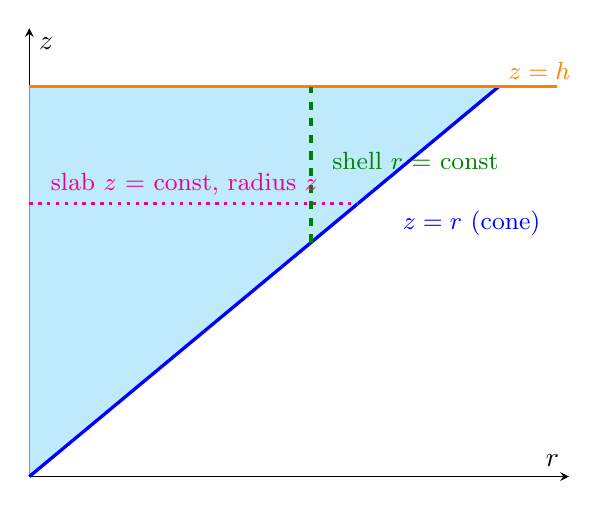
\begin{tikzpicture}
\begin{axis}[
    axis lines=middle,
    xlabel={$r$}, ylabel={$z$},
    xmin=0, xmax=2.3, ymin=0, ymax=2.3,
    ticks=none,
    clip=false]
    % Shaded region 0 <= r <= z <= h
    \addplot[fill=cyan!25, draw=none] coordinates {(0,0) (2,2) (0,2)};
    % Cone line z = r
    \addplot[very thick, blue, domain=0:2] {x};
    % Top z = h
    \addplot[very thick, orange, domain=0:2.25] {2};
    % Shell r = 1.2 (dashed green)
    \addplot[dashed, very thick, green!50!black] coordinates {(1.2,1.2) (1.2,2)};
    % Slab z = 1.4 (dotted magenta)
    \addplot[dotted, very thick, magenta] coordinates {(0,1.4) (1.4,1.4)};
    \node[green!50!black, anchor=west] at (axis cs:1.25,1.62) {\small shell $r$ = const};
    \node[magenta, anchor=west] at (axis cs:0.05,1.5) {\small slab $z$ = const, radius $z$};
    \node[blue, anchor=west] at (axis cs:1.55,1.3) {\small $z=r$ (cone)};
    \node[orange, anchor=west] at (axis cs:2.0,2.08) {\small $z=h$};
\end{axis}
\end{tikzpicture}
\end{document}